\documentclass[utf8]{ctexart}
\usepackage{graphicx}
\usepackage{amsmath, amssymb, amsthm}
\usepackage{geometry}
\usepackage{enumitem}
\usepackage{xcolor}
\usepackage{mdframed}
\usepackage{tikz}
\usetikzlibrary{graphs, positioning, arrows.meta}

\geometry{a4paper, margin=2.5cm}

% 定理环境
\newtheoremstyle{mystyle}
  {8pt}{8pt}{\kaishu}{0pt}{\bfseries}{}{1em}{}
\theoremstyle{mystyle}
\newtheorem{theorem}{定理}
\newtheorem{lemma}{引理}

% 好看的题目框
\newmdenv[
  linecolor=black!40,
  linewidth=1pt,
  backgroundcolor=gray!8,
  roundcorner=5pt,
  innertopmargin=8pt,
  innerbottommargin=8pt,
]{problembox}

\title{\textbf{离散数学2\quad 作业2}}
\date{\today}
\author{李子嘉 2024012325}
\begin{document}
\maketitle

\section*{题目1}

\begin{problembox}
判断以下四个邻接矩阵的简单图是否同构：
\[
A=
\begin{bmatrix}
0 & 1 & 0 & 1\\
1 & 0 & 0 & 1\\
0 & 0 & 0 & 1\\
1 & 1 & 1 & 0
\end{bmatrix},\qquad
B=
\begin{bmatrix}
0 & 1 & 1 & 1\\
1 & 0 & 0 & 1\\
1 & 0 & 0 & 1\\
1 & 1 & 1 & 0
\end{bmatrix}
\]

\[
C=
\begin{bmatrix}
0 & 1 & 1 & 0\\
1 & 0 & 0 & 1\\
1 & 0 & 0 & 1\\
0 & 1 & 1 & 0
\end{bmatrix},\qquad
D=
\begin{bmatrix}
0 & 1 & 0 & 1\\
1 & 0 & 0 & 0\\
0 & 0 & 0 & 1\\
1 & 0 & 1 & 0
\end{bmatrix}
\]
\end{problembox}

首先计算每个图的边数：A有4条边，B有5条边，C有4条边，D有3条边。
由于AC和B、D的边数不同，所以它们不可能同构。我们只需比较A和C是否同构。
A的度数序列为(2, 2, 1, 3)，C的度数序列为(2, 2, 2, 2)，因此A和C也不可能同构。
综上所述，这四个图两两不相同构。

\section*{题目2}
\begin{problembox}
  写出图1.25(a)的邻接矩阵、关联矩阵、边列表及正向表。
\end{problembox}
图1.25(a)的邻接矩阵为：
\[
\begin{bmatrix}
0 & 1 & 0 & 1 & 0 & 0\\
0 & 0 & 0 & 0 & 1 & 0\\
1 & 0 & 0 & 1 & 0 & 0\\
0 & 0 & 0 & 0 & 0 & 0\\
0 & 0 & 1 & 0 & 0 & 0\\
1 & 0 & 1 & 1 & 0 & 0
\end{bmatrix}
\]
关联矩阵为：
\[
\begin{bmatrix}
  1 & 1 & 0 & -1 & 0 & 0 & -1 & 0 & 0 \\
  -1 & 0 & 1 & 0 & 0 & 0 & 0 & 0 & 0 \\
  0 & 0 & 0 & 1 & 1 & -1 & 0 & -1 & 0 \\
  0 & -1 & 0 & 0 & -1 & 0 & 0 & 0 & -1 \\
  0 & 0 & -1 & 0 & 0 & 1 & 0 & 0 & 0 \\
  0 & 0 & 0 & 0 & 0 & 0 & 1 & 1 & 1
\end{bmatrix}
\]
边列表为：
\[
\begin{bmatrix}
  1 & 1 & 2 & 3 & 3 & 5 & 6 & 6 & 6 \\
  2 & 4 & 5 & 1 & 4 & 3 & 1 & 3 & 4
\end{bmatrix}
\]
正向表为：
\begin{center}
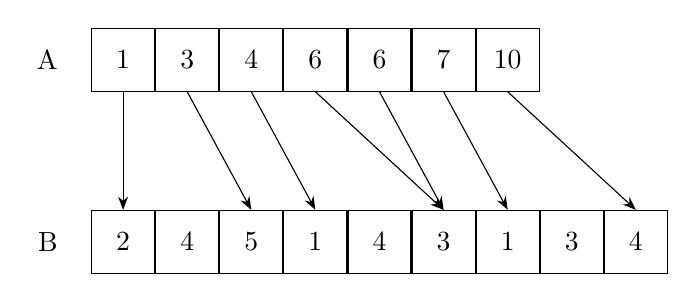
\begin{tikzpicture}[
node distance=0mm,
box/.style={draw, minimum width=8mm, minimum height=8mm, anchor=center},
>=Stealth
]

% A array
\node[box] (a0) {1};
\node[box, right=of a0] (a1) {3};
\node[box, right=of a1] (a2) {4};
\node[box, right=of a2] (a3) {6};
\node[box, right=of a3] (a4) {6};
\node[box, right=of a4] (a5) {7};
\node[box, right=of a5] (a6) {10};

\node[left=3mm of a0] {A};

% B array
\node[box, below=15mm of a0] (b1) {2};
\node[box, right=of b1] (b2) {4};
\node[box, right=of b2] (b3) {5};
\node[box, right=of b3] (b4) {1};
\node[box, right=of b4] (b5) {4};
\node[box, right=of b5] (b6) {3};
\node[box, right=of b6] (b7) {1};
\node[box, right=of b7] (b8) {3};
\node[box, right=of b8] (b9) {4};

\node[left=3mm of b1] {B};

% arrows
\draw[->] (a0.south) -- (b1.north);
\draw[->] (a1.south) -- (b3.north);
\draw[->] (a2.south) -- (b4.north);
\draw[->] (a3.south) -- (b6.north);
\draw[->] (a4.south) -- (b6.north);
\draw[->] (a5.south) -- (b7.north);
\draw[->] (a6.south) -- (b9.north);

\end{tikzpicture}
\end{center}

\section*{题目3}
\begin{problembox}
  判断图1.25是否同构。
\end{problembox}
是同构的，以下是各自节点的对应关系：

\[
\begin{aligned}
  V_1 &\leftrightarrow b \\
  V_2 &\leftrightarrow a \\
  V_3 &\leftrightarrow c \\
  V_4 &\leftrightarrow e \\
  V_5 &\leftrightarrow d \\
  V_6 &\leftrightarrow f
\end{aligned}
\]
\section*{题目4}
\begin{problembox}
  表示一个有n个顶点，m条边的非赋权图需要多少存储空间？其中分别利用：
  \begin{itemize}
    \item 邻接矩阵
    \item 关联矩阵
    \item 边列表
    \item 正向表
  \end{itemize}
\end{problembox}
\begin{itemize}
  \item 邻接矩阵需要存储$n^2$个元素，每个元素占用1个单位的存储空间，因此总共需要$n^2$个单位的存储空间。
  \item 关联矩阵需要存储$n \times m$个元素，每个元素占用1个单位的存储空间，因此总共需要$n \times m$个单位的存储空间。
  \item 边列表需要存储$m$条边，每条边由两个顶点组成，因此总共需要$2m$个单位的存储空间。
  \item 正向表有两个数组，数组A有n+1个元素，数组B有m个元素，因此总共需要$n+m+1$个单位的存储空间。
\end{itemize}
值得注意的是，邻接矩阵在无权图中可以使用布尔值来表示边的存在与否，因此每个元素最少可以只占1字节，而其余矩阵都至少需要int类型，也就是4字节。另外，不同存储结构访问图信息
所需要的时间也不一致，这涉及到空间换时间的问题。总的来说，一般稀疏图（m较小）时使用正向表/邻接表，而稠密图时使用邻接矩阵。

\end{document}